\section{Applications of Integration}

    \subsection{Average Value of a Function and Mean Value Theorem}
        The \color{purple}\textbf{average value }\color{black} of a function $f(x)$ over the
        interval $[a,b]$ is given by

        \begin{equation*}
            f_{avg} = \frac{1}{b-a}\int^b_a f(x)dx
        \end{equation*}

        \noindent \color{purple} \textbf{Mean Value Theorem}\color{black}: \\
        \noindent if $f(x)$ is a continuous function on $[a,b]$, then there is a number $c$ such
        that

        \begin{equation*}
            \int^b_a f(x)dx = f(c)(b-a)
        \end{equation*}

        \noindent \color{blue} \textit{Example 1: Find the average value of the function
        $f(x)=\sin{(2x)}e^{1-\cos{(2x)}}$ on $[-\pi,\pi]$}. \color{black}

        \begin{align*}
            u           &= 1-\cos{(2x)} \\
            f(x)_{avg}  &= \frac{1}{\pi-(-\pi)}\int^\pi_{-\pi}\sin{(2x)}e^{1-\cos{(2x)}}dx \\
            &= \frac{e^{1-\cos{2x}}}{4\pi}\Bigg|^\pi_{-\pi} \\
            &= 0
        \end{align*}

        \noindent \color{blue} \textit{Example 2: Find the number $c$ that satisfies the
        Mean Value Theorem for the function $f(x)=x^2+3x+2$ on $[1,4]$} \color{black}

        \noindent Notice that the function is a polynomial, hence it is continuous on the given
        interval and we can use the Mean Value Theorem.

        \begin{align*}
            \int^4_1 x^2+3x+2 dx                                    &= (c^2+3c+2)(4-1) \\
            \left(\frac{x^3}{3}+\frac{3x^2}{2}+2x\right)\Bigg^4_1   &= 3(c^2+3c+2) \\
            \frac{99}{2}                                            &= 3c^2+9c+6 \\
            0                                                       &= 3c^2+9c-\frac{87}{2} \\
            c                                                       &= 2.593,-5.593 \\
            \because c\in[1,4]                                      &\therefore c=2.593
        \end{align*}


    \subsection{Motion}
        Let the function $p(t)$ represent the position of a moving particle, with respect to
        time. Let the functions $v(t)$ and $a(t)$ represent the velocity and acceleration
        of the moving particle modeled by $p(t)$, respectively. Then the following equalities
        hold true:

        \begin{align*}
            \int a(t) &= v(t) + C \\
            \int v(t) &= p(t) + C
        \end{align*}

    \pagebreak
    \subsection{Areas between Curves}
        \color{purple} \textbf{Area Between Two Curves} \color{black}

        \begin{align*}
            A   &= \int^b_a (f(x)-g(x)) dx, a\leq x\leq b \\
            A   &= \int^d_c (f(y)-g(y)) dy, c\leq y\leq d
        \end{align*}

        \noindent where $f(x)$ is the upper function, $g(x)$ is the lower function,
        $f(y)$ is the right function, and $g(y)$ is the left function.

        \begin{figure}[hbt!]
            \centering
            \begin{subfigure}[b]{.45\textwidth}
                \includegraphics[scale=0.8]{Resources/Unit5IntegrationApps/Area1}
            \end{subfigure}
            \begin{subfigure}[b]{.45\textwidth}
                \includegraphics[scale=0.8]{Resources/Unit5IntegrationApps/Area2}
            \end{subfigure}
        \end{figure}

        \noindent \color{blue} \textit{Example 1: Find the area of the region enclosed by
        $y=x^2$ and $y=\sqrt{x}$} \color{black} \\

        \noindent Below is a graph for visual reference.

        \begin{figure}[hbt!]
            \centering
            \includegraphics[scale=0.75]{Resources/Unit5IntegrationApps/Area3}
        \end{figure}

        \begin{align*}
            A &= \int^1_0 (\sqrt{x}-x^2)dx \\
            &= \left(\frac{2}{3}x^{\frac{3}{2}}-\frac{1}{3}x^3\right)\Bigg|^1_0 \\
            &= \frac{1}{3}
        \end{align*}

        \noindent \color{blue} \texit{Example 2: Determine the area of the region bounded by
        $y=\sin{x},y=\cos{x},x=\frac{\pi}{2}$, and the $y$-axis.} \color{black} \\

        \noindent Below is a graph for reference. \\

        \begin{figure}[hbt!]
            \centering
            \includegraphics[scale=0.75]{Resources/Unit5IntegrationApps/Area4}
        \end{figure}

        \noindent The intersection point is given by $x=\sin{x}=\cos{x}=\frac{\pi}{4}$. Thus,

        \begin{align*}
            A   &= \int^{\frac{\pi}{4}}_0 (\cos{x}-\sin{x})dx
            + \int^{\frac{\pi}{2}}_{\frac{\pi}{4}}(\sin{x}-\cos{x})dx \\
            &= (\sin{x}+\cos{x})\Big|^{\frac{\pi}{4}}_0
            + (-\cos{x}-\sin{x})\Big|^\frac{\pi}{2}_{\frac{\pi}{4}} \\
            &= 2\sqrt{2}-2 \\
            &= 0.828427
        \end{align*}



    \subsection{Volumes with Cross Sections}
        \color{purple} \textbf{Volumes with Cross Sections} \color{black}
        \begin{equation*}
            V   &= \int^b_a A(y)dy
        \end{equation*}

        \noindent To determine the function $A(y)$ we must first express $A$ in terms of $x$. \\

        \noindent \color{blue} \textit{Example: The base of a solid $S$ is the region
        bounded by the parabola $x^2=8y$ and the line $y=4$. Use semi-circle cross-sections
        perpendicular to the $y$-axis to find the exact volume of solid $S$.} \color{black} \\

        \noindent Let us first graph the base of the solid. The orange rectangle represents a
        single cross-section sitting on the base. The length of the orange rectangle is $2x$.

        \begin{figure}[hbt!]
            \centering
            \includegraphics[scale=0.75]{Resources/Unit5IntegrationApps/Volume1}
        \end{figure}

        \noindent Because the semi-circle cross-section rests on the orange rectangle above,
        the diameter of the semi-circle is $2x$ and the radius is $x$. Thus, the area, $A$,
        of the semi-circle is given by

        \begin{equation*}
            A   = \frac{\pi}{2}x^2
        \end{equation*}

        \noindent Since the rectangle lies on the curve $x^2=8y$, we can write the area as

        \begin{equation*}
            A(y)    = \frac{\pi}{2}(8y) = 4\pi y
        \end{equation*}

        \noindent Then the volume, $V$, is

        \begin{align*}
            V &= \int^b_a A(y)dy \\
            &= 4\pi \int^4_0 ydy \\
            &= 4\pi\left[\frac{1}{2}y^2\right]^4_0 \\
            &= 32 \pi
        \end{align*}


    \pagebreak
    \subsection{Volumes with Disk Method}
        Say we have a function $y=f(x)$ like so:

        \begin{figure}[hbt!]
            \centering
            \begin{subfigure}[b]{.45\textwidth}
                \includegraphics[scale=0.8]{Resources/Unit5IntegrationApps/Disc1}
            \end{subfigure}
            \begin{subfigure}[b]{.45\textwidth}
                \includegraphics[scale=0.8]{Resources/Unit5IntegrationApps/Disc2}
            \end{subfigure}
        \end{figure}

        \noindent We can find the solid of revolution by adding up the infinitesimal discs
        (circles) on the interval. Notice that the volume of each disc is the area of its face
        multiplied by $dx$, the thickness of the disc. We know that the area of a circle is
        given by $A=\pi r^2$. Since the radius $r$ is the value of the function $f(x)$ at $x$,
        $A=\pi f(x)^2$. Then the volume of the solid of revolution is found by summing all the
        disks. Hence,

        \begin{equation*}
            V = \pi\int^b_a f(x)^2 dx
        \end{equation*}

        \noindent \color{blue} \textit{Example: Let a region be enclosed by the line
        $x=1$, the line $y=2$, the line $y=4$, and the curve $y=(x-1)^2$. A solid, $S$, is generated
        by rotating $R$ about the line $x=1$. Find the volume of the solid.} \color{black} \\

        \noindent Below is a graph depicting $R$, the shaded region, its bounds, and a single
        disk of the solid generated by revolving $R$ about $x=1$.

        \begin{figure}[hbt!]
            \centering
            \includegraphics[scale=0.75]{Resources/Unit5IntegrationApps/Disc3}
        \end{figure}

        \noindent Let us first find the radius of the discs, given by the distance between the
        curve $y=(x-1)^2$ and the line $x=1$. Rearranging the equation of the curve, we get
        $x=\sqrt{y}+1$. Then the radius, $r(y)$, is given by

        \begin{align*}
            r(y)    &= (\sqrt{y}+1)-(1) \\
            &= \sqrt{y}
        \end{align*}

        \noindent And the area of the disk's faces is given by
        \begin{align*}
            \pi[r(y)]^2 &= \pi(\sqrt{y})^2 \\
            &= \pi y
        \end{align*}

        \noindent Since the solid is bounded by the lines $y=2$ and $y=4$, the interval of
        integration is $[2,4]$. Then the volume of solid $S$ is given by

        \begin{align*}
            A &= \pi\int^4_2 ydy \\
            &= 6\pi
        \end{align*}


    \pagebreak
    \subsection{Volumes with Washer Method}
        A washer is a disk with a hole in its center. Say we have an outside function, $f(x)$,
        and an inside function, $g(x)$, like below.

        \begin{center}
            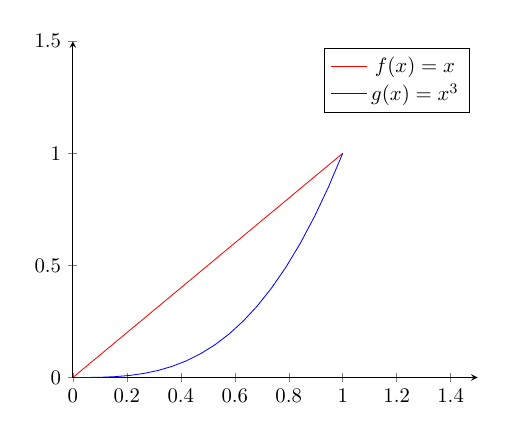
\begin{tikzpicture}[scale=0.75]
                \begin{axis}[
                    axis lines = left,
                    xmin = 0,
                    xmax = 1.5,
                    ymin = 0,
                    ymax = 1.5
                ]
                %f(x)
                \addplot [
                    samples = 2,
                    color = red,
                    domain = 0:1
                ]
                {x};
                \addlegendentry{$f(x)=x$}
                %g(x)
                \addplot [
                    samples = 20,
                    color = blue,
                    domain = 0:1
                ]
                {x^3};
                \addlegendentry{$g(x)=x^3$}
                \end{axis}
            \end{tikzpicture}
        \end{center}

        \noindent If we revolve $f(x)$ and $g(x)$ about the $x$-axis, we get a solid that looks
        like the one below. We can then imagine that the solid's volume is composed of
        infinitesimal washers that have radii of the outside function's radius minus the inside
        function's radius such that the washer's radius is $r(x)=f(x)-g(x)$ or $r(y)=f(y)-g(y)$.
        The area of each washer's face is given by

        \begin{equation*}
            A = \pi((\text{outer radius})^2-(\text{inner radius})^2)
        \end{equation*}

        \begin{figure}[hbt!]
            \centering
            \includegraphics[scale=0.75]{Resources/Unit5IntegrationApps/Washer1}
        \end{figure}

        \noindent Then we can find the volume of the solid of revolution by adding up the
        volumes of the disks found by multiplying their face areas by their widths, $dx$. The
        volume of the solid is then given by

        \begin{align*}
            V   &= \pi\int^b_a [f(x)^2-g(x)^2]dx
        \end{align*}

        \noindent \color{blue} \textit{Example: Find the volume of the solid generated by
        revolving the region bounded by the curves $y=x^2$ and $x=y^3$ about the line $x=-1$}
        \color{black} \\

        \noindent Below is a graph of the outside function $f(x)$ and the inner function $g(x)$
        for reference. The green region depicts the face area of a washer. We make the curve
        that is further away from the axis of revolution the outside function, and the curve
        closest to the axis of revolution the inner function.
        Note that the outside function, $f(x)=x^2$ has been rearranged to be
        $f(y)= y^{\frac{1}{2}}$. We then subtract "-1" from $f(y)$ and $g(y)$ to express the
        distance from the line of revolution, $x=-1$. Then the outside ($R(y)$) and inside
        ($r(y)$) radii are given by $R(y)=y^\frac{1}{2}+1$ and $r(y)=y^3+1$.

        \begin{center}
            \begin{tikzpicture}
                \begin{axis} [
                    axis lines = center,
                    xmin = -1.75,
                    xmax = 1.75,
                    ymin = -1.75,
                    ymax = 1.75
                ]
                % f(y)
                \addplot [
                    samples = 20,
                    color = red,
                    domain = -1.25:1.25,
                    name path = A
                ]
                {x^2};
                \addlegendentry{$R(y)=y^\frac{1}{2}+1$};
                % g(y)
                \addplot [
                    name path = B
                ]
                expression [
                    domain=-1.25:1.25,
                    samples=100,
                    color = blue
                ]
                {x/abs(x)*abs(x)^(1/3)};
                \addlegendentry{$r(y)=y^3+1$};
                % Line of revolution
                \draw [dashed] (-1,1.5) -- (-1,-1.2);
                % Area
                \addplot[
                    color = green,
                ]
                fill between [of=A and B, soft clip={domain=0:1.25}];
                \end{axis}
            \end{tikzpicture}
        \end{center}

        \noindent Then the volume of the solid of revolution is

        \begin{align*}
            V &= \pi\int^b_a[(R(y))^2-(r(y))^2]dy \\
            &= \pi\int^1_0[(y^\frac{1}{2}+1)^2 - (y^3+1)^2]dy \\
            &= \frac{25\pi}{21}
        \end{align*}

    \pagebreak
    \subsection{Arc Length}
        \color{purple} \textbf{The General Arc Length Formulae:} \color{black} \\

        \noindent The arc length, $L$, of a function on a continuous interval is given by

        \begin{equation*}
            L = \int^b_a ds
        \end{equation*}

        \noindent where

        \begin{align*}
            ds &= \sqrt{1+\left(\frac{dy}{dx}\right)^2}dx \text{ if } y=f(x),a\leq x\leq b \\
            ds &= \sqrt{1+\left(\frac{dx}{dy}\right)^2}dy \text{ if } x=g(y),a\leq y\leq b
        \end{align*}

        \noindent \color{purple} \textbf{Arc Length Formula for Parametric Equations} \color{black} \\

        \noindent For two functions $x=f(t)$ and $y=g(t), \alpha\leq t\leq \Beta$, the arc length
        of the parameterized curve is given by

        \begin{align*}
            L &= \int^\beta_\alpha \sqrt{\left(\frac{dx}{dt}\right)^2}dt
        \end{align*}

        \noindent \color{purple} \textbf{Arc Length Formula for Vector-Valued Functions} \color{black} \\

        \noindent For two vector-valued functions, $x=f(t),y=g(t)$, the arc length of the curve
        they form is given by

        \begin{align*}
            L   &= \int^b_a \| \overrightarrow{r}'(t)\| dt
        \end{align*}

        \noindent where $\|\overrightarrow{r}'(t)\|$ is the magnitude of the tangent vector such
        that

        \begin{align*}
            \|\overrightarrow{r}'(t)\|    &= \sqrt{[f'(t)]^2+[g'(t)]^2}
        \end{align*}